\subsection{Intrusion Detection Systems / Intrusion Prevention Systems}
Datensicherheit beschreibt eine Herangehensweise, das in erster Linie das Ziel verfolgt, ein System gegen vielzählige Verstöße zu schützen. Dies ist in den meisten Fällen nur schwer möglich, da die Systeme sehr komplex sein können. So gut wie jedes System weißt Sicherheitsschwachstellen auf, welche zu schwerläufigen Problemen führen können.
Als Antwort auf diese Sicherheitsprobleme, welche die Funktionsweise des Systems beinträchtigen können, etablierte sich eine neue Vorangehensweise. Die sogenanten Intrusion Detection Systems.
IDS überwachen Systeme auf eventuelle Sicherheitsverstöße und automatisieren die Analyseprozesse von Ereignissen. Somit können plötzliche Sicherheitsprobleme aufgedeckt werden.\cite{haystack_ids}
Grundsätzlich können Intrusion Detection Systems in 2 Hauptkategorien eingeteilt werden. Host-based und Network-based IDS.\cite{IDS_Book_1}

In diesem Abschnitt wird generell erklärt, was Host-basierte und Netzwerk-basierte Intrusion Detection Systems sind, mit einigen Beispiele.

\subsection{Host-based Intrusion Detection Systems}
HIDS (Host basierten IDS) setzen den Fokus auf die Aktivitäten eines einzigen Hosts. Sie fügen verletzlichen oder sensitiven Systemen, wie Datenbank-Servern oder administrativen Systemen, eine spezielle Sicherheits-Ebene hinzu. Das HIDS überwacht, auf versch. Art und Weise, Aktivitäten auf dem System. In einigen Fällen kann somit ein Angriff aufehalten werden, bevor er überhaupt Schaden verursacht. \cite{IDS_Book_1} \cite{IDS_Book_2}
Die Hauptaufgabe eines HIDS ist es, mit Regeln und Richtlinien, Protokolldateien zu durchsuchen und diese zu markieren, falls potentiell bösartige Verhaltensmuster erkennt werden.

HIDS können eine weitreichende Menge an Bedrohungen identifizieren. Dazu gehören:\cite{hids_url_2}

\begin{itemize}
  \item Unautorisiertes Einloggen und Zugriffsversuche
  \item Installation von unerwünschten Anwendungen
  \item Privileg-Eskalation
  \item Rogue-Processes
  \item Modifizieren der Binärdaten, Daten und Konfigurationsdateien von Anwendungen
  \item Kritische Dienste die gestoppt wurden oder nicht gestartet werde konnten
\end{itemize}

Der primäre Vorteil von HIDS ist diese interne und externe Bedrohungen identifizieren können, was nicht mit NIDS oder Firewalls möglich wäre.

Ein fundamentaler Bestandteil der Intrusion Detection ist der Sensor, der bestimmte Daten sammelt und diese zum Analysieren an das IDS weiterleitet. Das Thema Sensoren wird in einem späteren Abschnitt genauer erläutert.

Die meisten HIDS nutzen einen Kombination aus Signatur/Heuristik basierten und Anomalie basierten IDS.\cite{hids_url_1}
\textbf{Signatur/Heuristik basierte IDS} suchen nach ihnen schon bekannten Mustern, Identitäten oder spezifische Intrusion-Events, welche über eine Datenbank erkannt werden.\cite{hids_url_1}
\textbf{Anomalie basierte IDS} sind im Gegensatz zu den Signatur basierten IDS mehr auf die Analyse von vertrauenswürdigen Verhalten basiert. Hierzu wird Machine Learning genutzt um bösartiges Verhalten zu markieren.\cite{hids_url_1}

\subsection{Network-based IDS}
Network-based IDS hingegen analisieren Packete die direkt vom Netzwerk empfangen wurden. Durch das einsetzen von sogenannten Netzwerkkarten kann ein N-IDS den Netzwerkverkehr überwachen und somit alle Hosts schützen, die mit diesem Netzwerk verbunden sind.\cite{IDS_1}

\subsubsection{Snort}:
Snort ist ein vollständig ausgestattetes open-source Intrusion Prevention System\cite{snort_url}. Kurzgesagt handelt es sich bei Snort um einen "Packet Sniffer" (dt. Paketschnüffler) oder "Packetlogger". 
1998 schrieb Marty Roesch ein Packet Sniffer names APE, zu der Zeit nur für Linuxsysteme. Trotz der tollen Funktionalitäten wollte Roesch einen Sniffer erschaffen, der zudem folgende zusätzliche Eigenschaften haben sollte:\cite{snort_book_1}

\begin{itemize}
  \item funktioniert auf mehreren Betriebssystemen
  \item nutzt einen sog. hexdump payload dump
  \item zeigt alle untersch. Netzwerkpakete auf die selbe Weise an
\end{itemize}

Zu diesem Zeitpunkt wurde Snort nur für Packet-Sniffing genutzt. Roesch nutzt das Tool um seine Modem-Verbindung zu überwachen und seine eigenen Netzwerkanwendung zu debuggen. 1999 wurde Snort dann um eine Signatur-basierte Analyse (oder Regelbasierte-Analyse) Funktionalität erweitert. Ab hier konnte es dann schon als leichtgewichtiges IDS eingesetzt werden.\cite{snort_book_1}

\subsection{Sensoren}

Wie vorhin schon erwähnt sammelt ein Sensor im Kontext der IDS Daten aus einer Datenquelle. Übliche Datenquellen sind: \cite{IDS_Book_2}

\begin{itemize}
    \item \textbf{System call traces}: Beinhalten Sequenzen von Systemaufrufen von Prozessen. \cite{IDS_Book_2}
    \item \textbf{Log-Dateien}: Die meisten Betriebssysteme besitzen Software die Informationen über Nutzeraktivitäten sammelt.\cite{IDS_Book_2}
    \item \textbf{Prüfsumme der Datenintegrität}: Eine Möglichkeit, Nutzeraktivität auf einem System zu identifizieren, ist es regelmäßig kritische Dateien auf Änderungen zu analysieren. Hierbei wird die aktuelle kryptographische Prüfsumme der Dateien mit schon zuvor bekannten, korrekten Prüfsummen verglichen.\cite{IDS_Book_2}
    \item \textbf{Registry Zugang}: Eine Methode die auf Windows-Systemen genutzt wird. Hierbei wird der Zugang auf die Registry überwacht.\cite{IDS_Book_2}
\end{itemize}

Nachdem die Daten gesammelt wurden, werden zuerst ungewollte Informationen ausgefiltert. Dannach werden die übrigen Informationen in einem standardisierten Format bereitgestellt und diese zuletzt an das IDS zur Analyse weitergereicht.\cite{IDS_Book_2}

Sensoren können in 2 verschiedenen Modi eingesetzt werden. Inline und passiv.\cite{IDS_Book_2}

\subsubsection{Inline Sensoren:}
Ein Inline-Sensor wird in das Netzwerksegment eingeführt um den Verkehr zu überwachen. Jeglicher Verkehr muss diesen Sensor passieren. Mit Inline-Sensnoren können Attacken blockiert werden sobald sie aufgespürt wurden. In so einem Fall führt das System gleichzeitig eine Intrusion Detection und eine Intrusion Prevention durch\cite{url_sensors}\cite{IDS_Book_2}

\subsubsection{Passive Sensoren:}
Normalerweise werden im Allgemeinen meist passive Sensoren genutzt. Im Gegensatz zu Inline-Sensoren überwachen diese nicht direkt den Netzwerk-Verkehr, sondern nur eine Kopie davon. Der eigentliche Verkehr passiert diesen Sensor nicht. Diese Vorgehen ist insgesamt effizienter als das von Inline-Sensoren, da hier kein zusätzlicher Bearbeitungsschritt hinzugefügt wird, der zur Paketverzögerung beiträgt.\cite{url_sensors}\cite{IDS_Book_2}

\begin{figure}
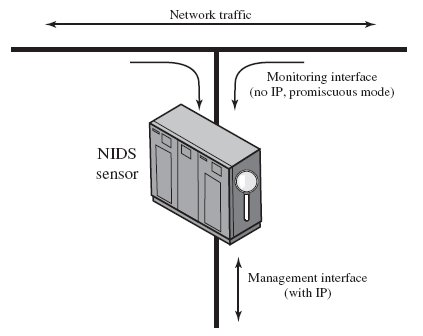
\includegraphics[width=\textwidth]{img/passive_sensor.jpg}
\caption{Illustration eines passiven NIDS Sensors} \label{fig1}
\end{figure}

\section{Eventuell Snort}